\documentclass{book}

\usepackage{amssymb}
\usepackage{amsmath}
\usepackage{amsthm}
\usepackage{arydshln}
\usepackage{calc}
\usepackage{cancel}
\usepackage{caption}
\usepackage{cite}
\usepackage{color}
\usepackage{enumitem}
\usepackage{esint}
\usepackage{etoolbox}
\usepackage{float}
\usepackage{framed}
\usepackage{fullpage}
\usepackage{gensymb}
\usepackage[margin=1in]{geometry}
\usepackage{graphicx}
\usepackage{listings}
\usepackage{multirow}
\usepackage{subfiles}
\usepackage{rsfso}
\usepackage{tikz}
\usepackage{tikz-3dplot}
\usepackage{ushort}
\usepackage{wrapfig}
\usepackage{xcolor}
\usepackage{soul}
\usepackage{epstopdf}
\usepackage{pgfplots}

% pdf versions
\pdfoptionpdfminorversion=7

% handle page stretching
\raggedbottom

% Graphics file location
\graphicspath{{Graphics/}{../Graphics/}}

% Use for drawings
\usetikzlibrary{angles,arrows,calc,decorations,intersections,patterns,positioning,quotes,shapes}
\usetikzlibrary{shapes.geometric}
\usetikzlibrary{decorations.pathreplacing}
\newcommand{\midarrow}{\tikz \draw[-latex] (0,0) -- +(.1,0);}

% Tikz commands for drawing block diagrams, etc...
\tikzset{%
	block/.style    = {draw, rectangle, minimum height = 2em, minimum width = 2em},
	sum/.style      = {draw, circle}, % Adder
	input/.style    = {fill=white, rectangle}, % Input
	output/.style   = {fill=white, rectangle}, % Output
	waypoint/.style   = {coordinate}, % Output
}

\tikzset{%
	startstop/.style= {draw, rectangle, rounded corners, minimum width=2cm, minimum height=1cm,text centered},
	inout/.style    = {draw, trapezium, trapezium left angle=70, trapezium right angle=110, minimum width=2cm, minimum height=1cm, text centered},
	process/.style  = {draw, rectangle, minimum width=2cm, minimum height=1cm, text centered},
	decision/.style = {draw, diamond, minimum width=1.5cm, minimum height=1cm, text centered, diamond, aspect=2},
	arrow/.style    = {thick,-latex,>=stealth},		
}

\tikzset{
	saveuse path/.code 2 args={
		\pgfkeysalso{#1/.style={insert path={#2}}}%
		\global\expandafter\let\csname pgfk@\pgfkeyscurrentpath/.@cmd\expandafter\endcsname
		% not optimal as it is now global through out the document
		\csname pgfk@\pgfkeyscurrentpath/.@cmd\endcsname
		\pgfkeysalso{#1}},
	/pgf/math set seed/.code=\pgfmathsetseed{#1}}

% Define Laplace, Fourier transform symbols
\newcommand{\LT}{\mathcal{L}}
\newcommand{\FT}{\mathcal{F}}

% Define adjugate function
\newcommand{\adj}{\text{adj}}

% Define rank function
\newcommand{\rank}{\text{rank}}

% commands to speed up writing j\omega and s-plane
\newcommand{\jw}{j\omega}
\newcommand{\spl}{s\textrm{-plane}}
\newcommand{\wt}{\omega t}
\newcommand{\Lm}{\textrm{Lm }}
% Clean up overline/underline for math mode
\def\obar#1{\bar{#1}}
\def\ubar#1{\ushort{#1}}

\newcommand{\exmp}{\subsubsection*{Example}}
\newcommand{\nib}{\noindent$ \bullet\ $}

% second-level itemize: change to circle
\renewcommand\labelitemii{$\circ$}


\begin{document}
	\chapter*{Lecture 13}

\section*{Frequency Response}
Designing controllers by frequency response is common in industry. We'll see it has some advantages over root locus design.

\begin{center}
	\begin{tikzpicture}[node distance = 3cm]
	\node[input] (in) {\begin{tikzpicture}[scale=0.25,domain=0:6.28]
		\draw[<->] (0,-2.25) -- (0,2.25);
		\draw[->] (0,0) -- (7,0) node[below left] {\footnotesize$ t $};
		\draw plot (\x,{1.5*sin(2*\x*(180/pi))});
		\end{tikzpicture}};
	\node[above of=in,node distance=0.75cm] {\footnotesize Input: $ u=A\sin(\wt)1(t) $};
	\node[block,right of=in,align=center] (sys) {LTI\\System};
	\node[output,right of=sys] (out) {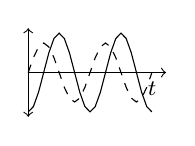
\begin{tikzpicture}[scale=0.25,domain=0:6.28]
		\draw[<->] (0,-2.25) -- (0,2.25);
		\draw[->] (0,0) -- (7,0) node[below left] {\footnotesize$ t $};
		\draw[dashed] plot (\x,{1.5*sin(2*\x*(180/pi))});
		\draw plot (\x,{2*sin(2*\x*(180/pi)-90)});
		\end{tikzpicture}};
	\node[above of=out,node distance=0.75cm] {\footnotesize Output: $ y_{ss}=B\sin(\wt+\phi)1(t) $};
	\draw[->] (in)--(sys);
	\draw[->] (sys)--(out);
	\end{tikzpicture}
\end{center}

We've spent a lot of time focusing on the case where the input is a step function. Now let's look at the case where the input is a sinusoid. Assume:

\begin{minipage}{0.55\textwidth}
	\[ u(t)=A\sin(\wt)\cdot1(t) \]
	Then,
	\[ \LT(u(t)) = U(s) = \frac{A\omega}{s^2+\omega^2} = \frac{A\omega}{(s+\jw)(s-\jw)} \]
	\[ Y(s) = GU = G\frac{A\omega}{(s+\jw)(s-\jw)} \]
	\[ Y = \frac{R_1}{s+\jw}+\frac{R_2}{s-\jw}+\text{extra terms from poles of }G(s) \]
	\[ y(t) = R_1 e^{-j\wt} + R_2 e^{j\wt} + \text{extra terms from poles of }G \]
\end{minipage}\hfill\vline\hfill
\begin{minipage}{0.4\textwidth}
	Reminder about period:
	\begin{itemize}
		\item $ \sin(t) $ is periodic with period $ T = 2\pi $
		\item If we replace $ t $ with $ \omega t $, then: $ \omega T = 2\pi $
		\item So, $ \sin(\wt) $ has a period of $ T=\frac{2\pi}{\omega} $
		
	\end{itemize}
\end{minipage}
\vspace{1em}

If $ G(s) $ is stable:
\begin{itemize}
	\item All poles of $ G(s) $ are in the LHP
	\item ``extra terms'' will decay to zero eventually
\end{itemize}
\[ y_{\text{steady state}}(t) = R_1 e^{-j\wt} + R_2 e^{j\wt} \]
We can find $ R_1 $ and $ R_2 $:
\[ R_1 = (s+\jw)Y\big|_{s=-\jw} = \left.\frac{G(s)A\omega}{s-\jw}\right|_{s=-\jw} = \frac{-AG(-\jw)}{2j} \]
\[ R_2 = (s-\jw)Y\big|_{s=\jw} = \left.\frac{G(s)A\omega}{s+\jw}\right|_{s=\jw} = \frac{AG(\jw)}{2j} \]
\[ \Rightarrow y_{ss}(t) = \frac{-AG(-\jw)}{2j} e^{-j\wt} + \frac{AG(\jw)}{2j} e^{j\wt} \]
What are $ G(\jw) $ and $ G(-\jw) $? We will use an example to show.

\exmp
Consider a system with transfer function $ G(s) = 3+s $. Find $ G(\jw) $ and $ G(-\jw) $ and evaluate at $ \omega=1,2,3 $.
\[ G(\jw) = 3+\jw,\quad G(-\jw) = 3-\jw \]
\[ \begin{array}{c c c}
\omega & G(\jw) & G(-\jw) \\ \hline
1 & 3+j & 3-j \\
2 & 3+2j & 3-2j \\
3 & 3+3j & 3-3j
\end{array} \]

\exmp
Consider a system with transfer function $ G(s) = (s+2)(s+4) $. Find $ G(\jw) $ and $ G(-\jw) $ and evaluate at $ \omega=1,2,3 $.
\[ G(s) = s^2+6s+8 \]
\[ G(\jw) = (\jw)^2+6(\jw)+8 = -\omega^2 + j6\omega + 8 = (8-\omega^2) + j(6\omega) \]
\[ G(-\jw) = (-\jw)^2-6(\jw)+8 = -\omega^2 - j6\omega + 8 = (8-\omega^2) - j(6\omega) \]
\[ \begin{array}{c c c}
\omega & G(\jw) & G(-\jw) \\ \hline
1 & 7+6j & 7-6j \\
2 & 4+12j & 4-12j \\
3 & -1+18j & -1-18j
\end{array} \]

In general: 
\[ G(\jw) = a(\omega) + jb(\omega) \]
\[ G(-\jw) = a(\omega) - jb(\omega) \]
Recall that a complex number can be written in polar notation as:
\[ a+jb = Me^{j\phi} \]
So,
\begin{center}
	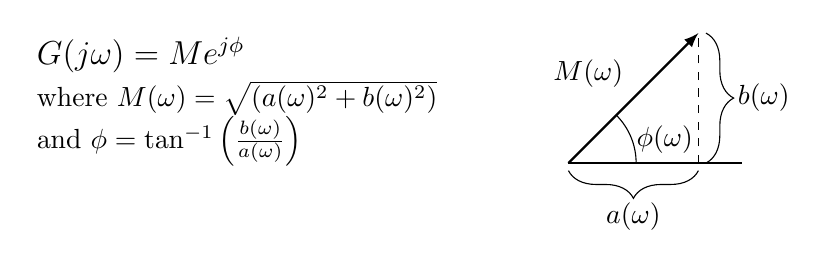
\begin{tikzpicture}[scale=1.375]
	\node[right] at (0, 0.4) {\large$ G(\jw)=Me^{j\phi} $};
	\node[right] at (0, 0) {where $ M(\omega)= \sqrt{(a(\omega)^2+b(\omega)^2)} $};
	\node[right] at (0, -0.4) {and $ \phi = \tan^{-1}\left( \frac{b(\omega)}{a(\omega)} \right) $};
	
	\draw[thick,-latex,xshift=1cm] (4,-0.6) -- node[above left] {$ M(\omega) $} (5.2,0.6);
	\draw[xshift=1cm] (4,-0.6) -- (5.6,-0.6);
	\draw[xshift=1cm] (4.625,-0.6) arc (0:45:0.625);
	\node[above right,xshift=1cm] at (4.8125,-0.6) {$ \phi(\omega) $};
	
	\draw [decorate,decoration={brace,amplitude=10pt,mirror}, xshift=1cm,yshift=-2pt]
	(4,-0.6) -- (5.2,-0.6)node [below,black,midway,yshift=-8pt] {$a(\omega)$};
	
	\draw [decorate,decoration={brace,amplitude=10pt,mirror}, xshift=2pt,yshift=0pt]
	(6.2,-0.6) -- (6.2,0.6)node [right,black,midway,xshift=8pt] {$b(\omega)$};
	
	\draw[dashed,xshift=1cm] (5.2,-0.6) -- (5.2,0.6);
	\end{tikzpicture}
\end{center}

\begin{center}
	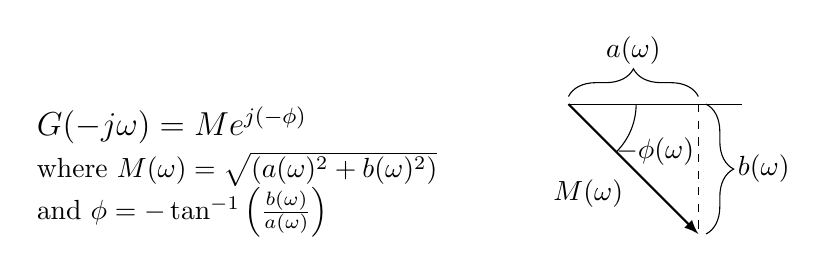
\begin{tikzpicture}[scale=1.375]
	\node[right] at (0, 0.4) {\large$ G(-\jw)=Me^{j(-\phi)} $};
	\node[right] at (0, 0) {where $ M(\omega)= \sqrt{(a(\omega)^2+b(\omega)^2)} $};
	\node[right] at (0, -0.4) {and $ \phi = -\tan^{-1}\left( \frac{b(\omega)}{a(\omega)} \right) $};
	
	\draw[thick,-latex,xshift=1cm] (4,0.6) -- node[below left] {$ M(\omega) $} (5.2,-0.6);
	\draw[xshift=1cm] (4,0.6) -- (5.6,0.6);
	\draw[xshift=1cm] (4.625,0.6) arc (0:-45:0.625);
	\node[right,xshift=1cm] at (4.625,0.16) {$ -\phi(\omega) $};
	
	\draw [decorate,decoration={brace,amplitude=10pt}, xshift=0pt,yshift=2pt]
	(5,0.6) -- (6.2,0.6) node [above,black,midway,yshift=8pt] {$a(\omega)$};
	
	\draw [decorate,decoration={brace,amplitude=10pt}, xshift=2pt,yshift=0pt]
	(6.2,0.6) -- (6.2,-0.6)node [right,black,midway,xshift=8pt] {$b(\omega)$};
	
	\draw[dashed,xshift=1cm] (5.2,0.6) -- (5.2,-0.6);
	\end{tikzpicture}
\end{center}

Now, we will substitute these definitions of $ G(\jw) $ and $ G(-\jw) $ into the definition of $ y_{ss}(t) $.
\[ y_{ss}(t) = \frac{-AG(-\jw)}{2j} e^{-j\wt} + \frac{AG(\jw)}{2j} e^{j\wt} \]
\[ y_{ss}(t) = \frac{-AMe^{-j\phi}}{2j} e^{-j\wt} + \frac{AMe^{j\phi}}{2j} e^{j\wt} \]
\[ y_{ss}(t) = \frac{-AM}{2j} e^{-j(\wt+\phi)} + \frac{AM}{2j} e^{j(\wt+\phi)} \]
\[ y_{ss}(t) = AM\left( \frac{e^{j(\wt+\phi)}-e^{-j(\wt+\phi)}}{2j} \right) \]
\[ \boxed{y_{ss}(t) = AM(\omega)\sin\left(\wt+\phi(\omega)\right)} \]
\begin{itemize}
	\item If the input is a sine wave, then the output at steady state is a sine wave.
	\item Frequency of input = frequency of output
	\item The output differs from the input in two ways:
	\begin{enumerate}
		\item Amplitude of output = Amplitude of input $ \times\ M(\omega) $
		\item There is a phase shift of $ \phi(\omega) $
	\end{enumerate}
	\item $ M(\omega) $ is the gain or Bode magnitude
	\item $ \phi(\omega) $ is the phase angle
\end{itemize}

\section*{Finding $ M $ and $ \phi $ from a transfer function}
\exmp
Find the expressions for $ G(\jw) $, $ M(\omega) $ and $ \phi(\omega) $ for $ G(s) = s+2 $.
\[ G(\jw)=2+\jw \]
\[ M(\omega) = \sqrt{2^2+\omega^2} \]
\[ \phi(\omega) = \tan^{-1}\left(\frac{\omega}{2}\right) \]

\exmp
Find the expressions for $ G(\jw) $, $ M(\omega) $ and $ \phi(\omega) $ for $ G(s) = (s+2)/(s+3) $.
\[ G(\jw)=\frac{\jw+2}{\jw+3}=\frac{M_1e^{j\phi_1}}{M_2e^{j\phi_2}}=\frac{M_1}{M_2}e^{j(\phi_1-\phi_2)} \]
\[ M(\omega) = \frac{\sqrt{2^2+\omega^2}}{\sqrt{3^2+\omega^2}} \]
\[ \phi(\omega) = \tan^{-1}\left(\frac{\omega}{2}\right) - \tan^{-1}\left(\frac{\omega}{3}\right) \]

\section*{Graphical representations of frequency response}
The frequency response is typically represented on a \textbf{Bode Diagram}, which includes two plots:
\begin{enumerate}
	\item[Plot 1:] Magnitude plot: $ 20\log_{10}M(\omega) $ in decibels vs. $ \omega $ in rad/s, where $ \omega $ is on a log scale.
	\item[Plot 2:] Phase plot: $ \phi $ in degrees vs. $ \omega $ in rad/s, where $ \omega $ is on a log scale.
\end{enumerate}

A few notes on log magnitude:
\begin{itemize}
	\item $ 20\log_{10}M $ is often written as $ \Lm M $ --- ``the log-magnitude of M''.
	\item Multiplication/division in the linear scale is equivalent to addition/subtraction in the dB scale.
	\item Some common magnitudes in linear and log scales:
		\[ \begin{array}{c c l}
			M=1 & \Rightarrow & \Lm M = 20\log_{10}(1) = 0\text{ dB}\\
			M=10 & \Rightarrow & \Lm M = 20\log_{10}(10) = 20\text{ dB}\\
			M=0.1 & \Rightarrow & \Lm M = 20\log_{10}(0.1) = -20\text{ dB}\\
			M=2 & \Rightarrow & \Lm M = 20\log_{10}(2) = 6\text{ dB}\\
			M=\frac{1}{2} & \Rightarrow & \Lm M = 20\log_{10}\left(\frac{1}{2}\right) = -6\text{ dB}\\
			M=\sqrt{2} & \Rightarrow & \Lm M = 20\log_{10}\left(\sqrt{2}\right) = 3\text{ dB}\\
		\end{array} \]
		Or, working backwards:
		\[ \begin{array}{c c l}
			\Lm M=0\text{ dB} & \Rightarrow & M = 10^{0/20} = 1\\
			\Lm M=20\text{ dB} & \Rightarrow & M = 10^{20/20} = 10\\
			\Lm M=-20\text{ dB} & \Rightarrow & M = 10^{-20/20} = 0.1\\
			\Lm M=6\text{ dB} & \Rightarrow & M = 10^{6/20} = 2\\
			\Lm M=-6\text{ dB} & \Rightarrow & M = 10^{-6/20} = \frac{1}{2}\\
			\Lm M=3\text{ dB} & \Rightarrow & M = 10^{3/20} = \sqrt{2}\\
			\end{array} \]
\end{itemize}

\exmp
Evaluate the log-magnitude of $ M=20 $.
\[ \Lm 20 = \Lm (10\cdot 2) = \Lm10 + \Lm2= 20+6 \]
\[ \Lm20  = 26\text{ dB} \]

Evaluate the log-magnitude of $ M=5\sqrt{2} $.
\[ \Lm 5\sqrt{2} = \Lm \left(10/\sqrt{2}\right) = \Lm10 - \Lm\sqrt{2} = 20-3 \]
\[ \Lm 5\sqrt{2} = 17\text{ dB} \]

\section*{Sketching Bode plots}
\paragraph{Note:} Before we begin, note that Bode plots are drawn on a \textbf{logarithmic} scale, not a linear one.
\begin{center}
	\begin{tikzpicture}[scale = 2]
		\draw (-3.5,0) -| (-3,-0.05) node[below] {-3} (-3,0) -| (-2,-0.05) node[below] {-2} (-2,0) -| (-1,-0.05) node[below] {-1} (-1,0) -| (0,-0.05) node[below] {0} (0,0) -| (1,-0.05) node[below] {1} (1,0) -| (2,-0.05) node[below] {2} (2,0) -| (3,-0.05) node[below] {3} (3,0) -- (3.5,0);
	\end{tikzpicture}\\
	Linear Scale \\
	
	\vspace{2em}
	
	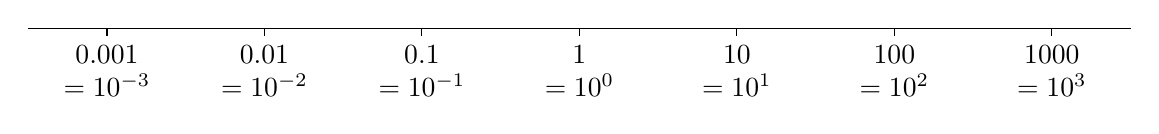
\begin{tikzpicture}[scale = 2]
	\draw (-3.5,0) -| (-3,-0.05) node[below, align=center] {$ 0.001 $ \\ $ = 10^{-3} $} (-3,0) -| (-2,-0.05) node[below, align=center] {$ 0.01 $ \\ $ =10^{-2} $} (-2,0) -| (-1,-0.05) node[below, align=center] {$ 0.1 $ \\ $ =10^{-1} $} (-1,0) -| (0,-0.05) node[below, align=center] {$ 1 $ \\ $ =10^{0} $} (0,0) -| (1,-0.05) node[below, align=center] {$ 10 $ \\ $ =10^{1} $} (1,0) -| (2,-0.05) node[below, align=center] {$ 100 $ \\ $ =10^{2} $} (2,0) -| (3,-0.05) node[below, align=center] {$ 1000 $ \\ $ =10^{3} $} (3,0) -- (3.5,0);
	\end{tikzpicture}\\
	Logarithmic Scale
\end{center}
Specifically, the x-axis is a logarithmic scale of the oscillation frequency $ \omega $. We refer to an increase of one power of 10 as a ``decade''. For instance, $ 10^0 $ to $ 10^1 $ is one decade; $ 10^2 $ to $ 10^3 $ is one decade; $ 10^{-2} $ to $ 10^0 $ is two decades, and so on.

\paragraph{Drawing Bode Plots:} 
If $ G(s) $ is a rational function, then it consists of terms such as: $ K $, $ 1/s $, $ s $, $ s+a $, $ 1/(s+a) $, $ \omega_n^2/(s^2+2\zeta\omega_ns+\omega_n^2) $, etc... Let's look at how to sketch Bode plots for these simple terms.

\paragraph*{Gain}
Let $ G(s) = K $. What is the Bode plot?
\[ G(\jw) = K+j(0) \]
\[ M(\omega) = K \]
\[ \phi(\omega) = \tan^{-1}\left(\frac{0}{K}\right)=0 \]

\begin{center}
	\hspace*{\fill}
	\begin{tikzpicture}[xscale=1.25]
		\draw[<->] (0,3) node[below left] {$\Lm M$} |- (4,0) node[below left] {$ \omega $};
		\draw (0,1.5) node[left] {$ 20\log_{10}(K) $} -- (4,1.5);
	\end{tikzpicture}
	\hfill
	\begin{tikzpicture}[xscale=1.25]
		\draw[<->] (0,3) node[below left] {$\phi$} |- (4,0) node[below left] {$ \omega $};
		\draw (0,1.5) node[left] {$ 0^\circ $} -- (4,1.5);
	\end{tikzpicture}
	\hspace*{\fill}
\end{center}

\paragraph*{Integrator}
Let $ G(s) = 1/s $. What is the Bode plot?
\[ G(\jw) = \frac{1}{\jw} \]
\[ M(\omega) = \frac{M_{num}}{M_{den}} = \frac{\sqrt{1^2+0^2}}{\sqrt{0^2+\omega^2}} = \frac{1}{\omega} \]
\[ \Lm M(\omega) = 20\log_{10} \frac{1}{\omega} = 20\log_{10}(1) - 20\log_{10} (\omega) = -20\log_{10} \omega \]
\[ \phi(\omega) = \phi_{num} - \phi_{den} =  \tan^{-1}\left(\frac{0}{1}\right) - \tan^{-1}\left(\frac{\omega}{0}\right) = 0 - 90^\circ = - 90^\circ \]

\begin{center}
	\hspace*{\fill}
	\begin{tikzpicture}[xscale=1.25]
		\draw[<->] (0,3.5) node[left] {$\Lm M$} |- (4,0) node[below left] {$ \omega $};		
		
		\foreach \x [evaluate=\x as \xeval using log10(\x)+1] in {0.1,1,10,100} \draw (\xeval cm,0pt) -- (\xeval cm,-2pt) node[anchor=north] {$\x$};
		
		\foreach \y [evaluate=\y as \yeval using (\y+40)/20] in {20,0,-20,-40} \draw (0pt,\yeval cm) -- (-2pt,\yeval cm) node[anchor=east] {$\y$};
		
		\draw (0,3) -- (3,0);
		\draw[dashed] (0,2) -| (1,0);
	\end{tikzpicture}
	\hfill
	\begin{tikzpicture}[xscale=1.25]
		\draw[<->] (0,3.5) node[left] {$\phi$} |- (4,0) node[below left] {$ \omega $};
		
		\foreach \x [evaluate=\x as \xeval using log10(\x)+1] in {0.1,1,10,100} \draw (\xeval cm,0pt) -- (\xeval cm,-2pt) node[anchor=north] {$\x$};
		
		\foreach \y [evaluate=\y as \yeval using (\y+180)/90] in {90,0,-90,-180} \draw (0pt,\yeval cm) -- (-2pt,\yeval cm) node[anchor=east] {$\y$};
		
		\draw (0,1) -- (4,1);
	\end{tikzpicture}
	\hspace*{\fill}
\end{center}

\paragraph*{Double Integrator}
Let $ G(s) = 1/s^2 $. What is the Bode plot?
\[ G(\jw) = \frac{1}{(\jw)^2} = \frac{1}{-\omega^2} \]
\[ M(\omega) = \frac{M_{num}}{M_{den}} = \frac{\sqrt{1^2+0^2}}{\sqrt{0^2+(-\omega^2)^2}} = \frac{1}{\omega^2} \]
\[ \Lm M(\omega) = 20\log_{10} \frac{1}{\omega^2} = 20\log_{10}(1) - 2\times20\log_{10} (\omega) = -40\log_{10} \omega \]
\[ \phi(\omega) = \phi_{num} - \phi_{den} =  \tan^{-1}\left(\frac{0}{1}\right) - \tan^{-1}\left(\frac{0}{-\omega^2}\right) = 0 - 180^\circ = - 180^\circ \]

\begin{center}
	\hspace*{\fill}
	\begin{tikzpicture}[xscale=1.25]
	\draw[<->] (0,3.5) node[left] {$\Lm M$} |- (4,0) node[below left] {$ \omega $};		
	
	\foreach \x [evaluate=\x as \xeval using log10(\x)+1] in {0.1,1,10,100} \draw (\xeval cm,0pt) -- (\xeval cm,-2pt) node[anchor=north] {$\x$};
	
	\foreach \y [evaluate=\y as \yeval using (\y+80)/40] in {40,0,-40,-80} \draw (0pt,\yeval cm) -- (-2pt,\yeval cm) node[anchor=east] {$\y$};
	
	\draw (0,3) -- (3,0);
	\draw[dashed] (0,2) -| (1,0);
	\end{tikzpicture}
	\hfill
	\begin{tikzpicture}[xscale=1.25]
	\draw[<->] (0,3.5) node[left] {$\phi$} |- (4,0) node[below left] {$ \omega $};
	
	\foreach \x [evaluate=\x as \xeval using log10(\x)+1] in {0.1,1,10,100} \draw (\xeval cm,0pt) -- (\xeval cm,-2pt) node[anchor=north] {$\x$};
	
	\foreach \y [evaluate=\y as \yeval using (\y+270)/90] in {0,-90,-180,-270} \draw (0pt,\yeval cm) -- (-2pt,\yeval cm) node[anchor=east] {$\y$};
	
	\draw (0,1) -- (4,1);
	\end{tikzpicture}
	\hspace*{\fill}
\end{center}

\paragraph*{Differentiator}
Let $ G(s) = s $. What is the Bode plot?
\[ G(\jw) = \jw \]
\[ M(\omega) = \sqrt{0^2+\omega^2} = \omega \]
\[ \phi(\omega) = \tan^{-1}\left(\frac{\omega}{0}\right) = 90^\circ \]

\begin{center}
	\hspace*{\fill}
	\begin{tikzpicture}[xscale=1.25]
	\draw[<->] (0,3.5) node[left] {$\Lm M$} |- (4,0) node[below left] {$ \omega $};
	
	\foreach \x [evaluate=\x as \xeval using log10(\x)+1] in {0.1,1,10,100} \draw (\xeval cm,0pt) -- (\xeval cm,-2pt) node[anchor=north] {$\x$};
	
	\foreach \y [evaluate=\y as \yeval using (\y+20)/20] in {40,20,0,-20} \draw (0pt,\yeval cm) -- (-2pt,\yeval cm) node[anchor=east] {$\y$};
	
	\draw (0,0) -- (3.5,3.5);
	\draw[dashed] (0,1) -| (1,0);
	\end{tikzpicture}
	\hfill
	\begin{tikzpicture}[xscale=1.25]
	\draw[<->] (0,3.5) node[left] {$\phi$} |- (4,0) node[below left] {$ \omega $};
	
	\foreach \x [evaluate=\x as \xeval using log10(\x)+1] in {0.1,1,10,100} \draw (\xeval cm,0pt) -- (\xeval cm,-2pt) node[anchor=north] {$\x$};
	
	\foreach \y [evaluate=\y as \yeval using (\y+90)/90] in {180,90,0,-90} \draw (0pt,\yeval cm) -- (-2pt,\yeval cm) node[anchor=east] {$\y$};
	
	\draw (0,2) -- (4,2);
	\end{tikzpicture}
	\hspace*{\fill}
\end{center}
The plot of $ s $ is a mirror image of the plot of $ 1/s $.

\paragraph*{First-Order Zero}
Let $ G(s) = \tau s+1 $. What is the Bode plot?
\[ G(\jw) = 1+j(\tau\omega) \]
\[ M(\omega) = \sqrt{1^2+\tau^2\omega^2}\]
\[ \phi(\omega) = \tan^{-1}\left(\frac{\tau\omega}{1}\right) \]
Neither the gain nor phase is a straight line. They will be harder to sketch than in previous cases. We will start by looking at the gain by finding:
\begin{itemize}
	\item an approximation for $ M $ when $ \tau\omega \ll 1 $,
	\item an approximation for $ M $ when $ \tau\omega \gg 1 $, and
	\item a precise value of $ M $ when $ \tau\omega = 1 $
\end{itemize}
When $ \tau\omega \ll 1 $: 
\begin{itemize}
	\item $ \tau\omega\approx0 $ so $ M(\omega) \approx 1 $.
	\item $ 20\log_{10}(1) = 0 $
\end{itemize}
When $ \tau\omega \gg 1 $: 
\begin{itemize}
	\item $ \tau\omega+1\approx\tau\omega $ so $ M(\omega) \approx \tau\omega $.
	\item $ 20\log_{10}(\tau\omega) $ is a straight line with slope of 20dB/decade and is 0 at $ \omega=1/\tau $.
\end{itemize}
When $ \tau\omega = 1 $ precisely:
\begin{itemize}
	\item $ M(\omega) = \sqrt{1+1} = \sqrt 2$.
	\item $ \Lm M(1/\tau) = 3 $dB.
\end{itemize}

\begin{center}
	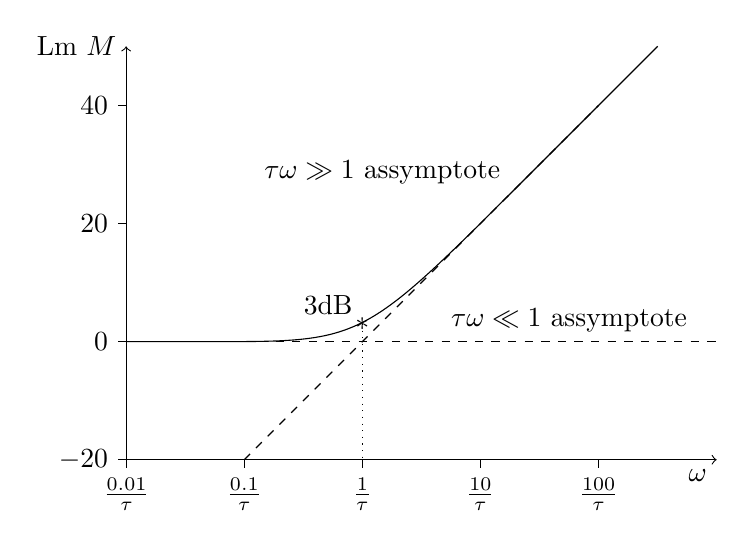
\begin{tikzpicture}[scale=1.5]
	\draw[<->] (0,3.5) node[left] {$\Lm M$} |- (5,0) node[below left] {$ \omega $};
	
	\foreach \x [evaluate=\x as \xeval using log10(\x)+2] in {0.01,0.1,1,10,100} \draw (\xeval cm,0pt) -- (\xeval cm,-2pt) node[anchor=north] {$\frac{\x}{\tau}$};
	
	\foreach \y [evaluate=\y as \yeval using (\y+20)/20] in {40,20,0,-20} \draw (0pt,\yeval cm) -- (-2pt,\yeval cm) node[anchor=east] {$\y$};
	
	\draw[dashed] (0,1) -- node[above,pos=0.75] {$ \tau\omega \ll 1 $ assymptote} (5,1);
	\draw[dashed] (1,0) -- node[above left,pos=0.75] {$ \tau\omega \gg 1 $ assymptote} (4,3);
	\draw[dotted] (2,1.15) node {$ * $} -- (2,0);
	\draw (0,1) -- (0.75,1) ..controls (2,1) .. (3.35,2.35) -- (4.5,3.5);
	\node[above left] at (2,1.15) {3dB};
	\end{tikzpicture}
\end{center}
Next, we look at the phase by finding approximations for $ \phi $ when::
\begin{itemize}
	\item an approximation for $ M $ when $ \tau\omega \ll 1 $,
	\item an approximation for $ M $ when $ \tau\omega \gg 1 $, and
	\item a precise value of $ M $ when $ \tau\omega = 1 $
\end{itemize}
When $ \tau\omega \ll 1 $: 
\begin{itemize}
	\item $ \tau\omega\approx0 $ so $ \phi(\omega) \approx \tan^{-1}(0/1)=0^\circ $.
\end{itemize}
When $ \tau\omega \gg 1 $: 
\begin{itemize}
	\item $ \tau\omega+1\approx\tau\omega $ and $ \tau\omega\approx\infty $ so $ \phi(\omega) \approx \tan^{-1}(\infty/1) = 90^\circ $.
\end{itemize}
When $ \tau\omega = 1 $ precisely:
\begin{itemize}
	\item $ \phi(\omega) = \tan^{-1}(1/1) = 45^\circ $.
\end{itemize}
\begin{center}
	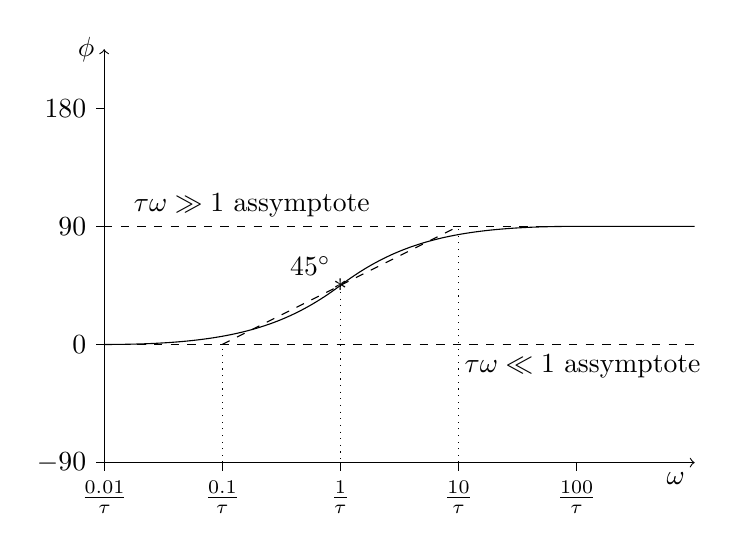
\begin{tikzpicture}[scale=1.5]
	\draw[<->] (0,3.5) node[left] {$\phi$} |- (5,0) node[below left] {$ \omega $};
	
	\foreach \x [evaluate=\x as \xeval using log10(\x)+2] in {0.01,0.1,1,10,100} \draw (\xeval cm,0pt) -- (\xeval cm,-2pt) node[anchor=north] {$\frac{\x}{\tau}$};
	
	\foreach \y [evaluate=\y as \yeval using (\y+90)/90] in {180,90,0,-90} \draw (0pt,\yeval cm) -- (-2pt,\yeval cm) node[anchor=east] {$\y$};
	
	\draw (0,1) ..controls (1,1) and (1.5,1.125) .. (2,1.5) ..controls (2.5,1.875) and (3,2) .. (4,2) -- (5,2);
	\draw[dashed] (0,1) -- node[below,pos=0.81] {$ \tau\omega \ll 1 $ assymptote} (5,1);
	\draw[dashed] (0,2) -- node[above,pos=0.25] {$ \tau\omega \gg 1 $ assymptote} (5,2);
	\draw[dotted] (1,0) -- (1,1);
	\draw[dotted] (3,0) -- (3,2);
	\draw[dotted] (2,1.5) node {$ * $} -- (2,0);
	\node[above left] at (2,1.5) {$ 45^\circ $};
	\draw[dashed] (1,1) -- (3,2);
	\end{tikzpicture}
\end{center}

A decent rule of thumb for drawing first-order phase plots is that the phase change takes place over roughly 2 decades, centered on the cutoff frequency (or $ 1/\tau $). This line is marked on the phase plot.

\paragraph*{First-Order Pole}
The first-order pole $ G(s) = 1/(\tau s+1) $ is a mirror image of the first-order zero.
\begin{center}
	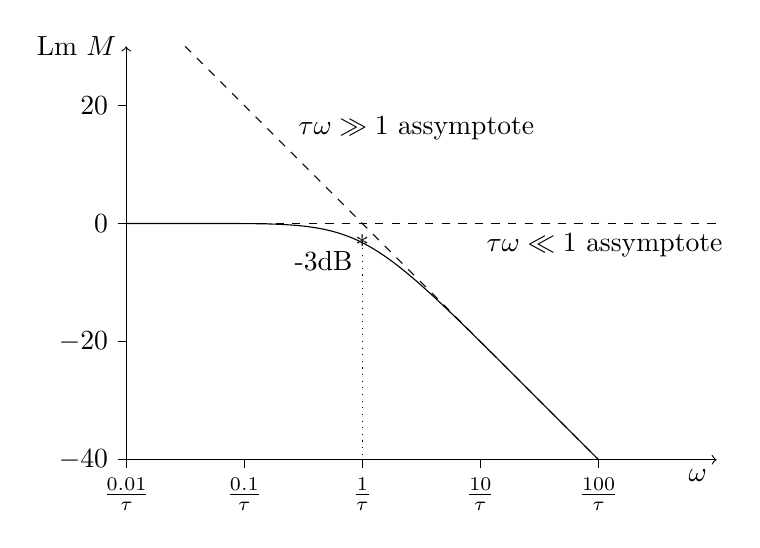
\begin{tikzpicture}[scale=1.5]
	\draw[<->] (0,3.5) node[left] {$\Lm M$} |- (5,0) node[below left] {$ \omega $};
	
	\foreach \x [evaluate=\x as \xeval using log10(\x)+2] in {0.01,0.1,1,10,100} \draw (\xeval cm,0pt) -- (\xeval cm,-2pt) node[anchor=north] {$\frac{\x}{\tau}$};
	
	\foreach \y [evaluate=\y as \yeval using (\y+40)/20] in {-40,20,0,-20} \draw (0pt,\yeval cm) -- (-2pt,\yeval cm) node[anchor=east] {$\y$};
	
	\draw[dashed] (0,2) -- node[below,pos=0.81] {$ \tau\omega \ll 1 $ assymptote} (5,2);
	\draw[dashed] (0.5,3.5) -- node[above right,pos=0.25] {$ \tau\omega \gg 1 $ assymptote} (4,0);
	\draw[dotted] (2,1.85) node {$ * $} -- (2,0);
	\draw (0,2) -- (0.75,2) ..controls (2,2) .. (3.35,0.65) -- (4,0);
	\node[below left] at (2,1.85) {-3dB};
	\end{tikzpicture}
\end{center}
\begin{center}
	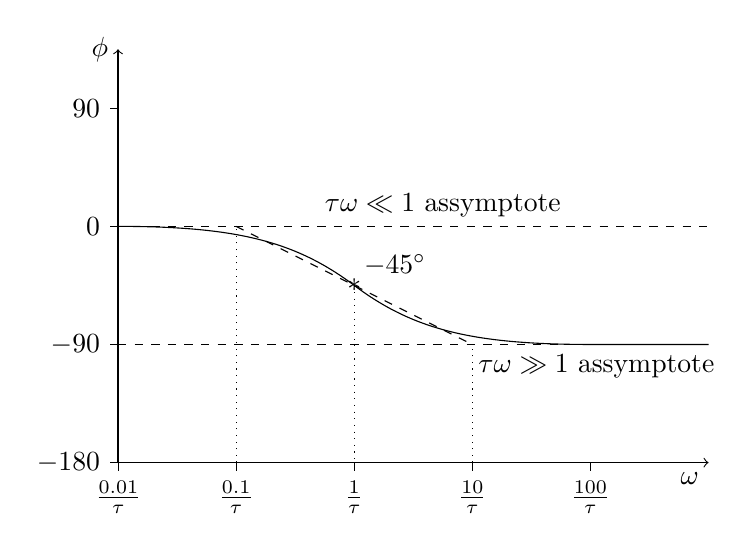
\begin{tikzpicture}[scale=1.5]
	\draw[<->] (0,3.5) node[left] {$\phi$} |- (5,0) node[below left] {$ \omega $};
	
	\foreach \x [evaluate=\x as \xeval using log10(\x)+2] in {0.01,0.1,1,10,100} \draw (\xeval cm,0pt) -- (\xeval cm,-2pt) node[anchor=north] {$\frac{\x}{\tau}$};
	
	\foreach \y [evaluate=\y as \yeval using (\y+180)/90] in {-180,90,0,-90} \draw (0pt,\yeval cm) -- (-2pt,\yeval cm) node[anchor=east] {$\y$};
	
	\draw (0,2) ..controls (1,2) and (1.5,1.875) .. (2,1.5) ..controls (2.5,1.125) and (3,1) .. (4,1) -- (5,1);
	\draw[dashed] (0,1) -- node[below,pos=0.81] {$ \tau\omega \gg 1 $ assymptote} (5,1);
	\draw[dashed] (0,2) -- node[above,pos=0.55] {$ \tau\omega \ll 1 $ assymptote} (5,2);
	\draw[dotted] (1,0) -- (1,2);
	\draw[dotted] (3,0) -- (3,1);
	\draw[dotted] (2,1.5) node {$ * $} -- (2,0);
	\node[above right] at (2,1.5) {$ -45^\circ $};
	\draw[dashed] (1,2) -- (3,1);
	\end{tikzpicture}
\end{center}

\paragraph*{Second-Order Pole}
Let $ G(s)$ be defined as
\[ G(s) = \frac{\omega_n^2}{s^2+2\zeta\omega_ns+\omega_n^2} \]
What is the Bode plot?
\[ G(\jw) = \frac{1}{\frac{-\omega^2}{\omega_n^2}+\frac{j(2\zeta \omega)}{\omega_n}+1} = \frac{1}{\left( 1-\frac{\omega^2}{\omega_n^2} \right) + j\left( 2\zeta\frac{\omega}{\omega_n} \right)} \]
We will start by finding the gain as a function of $ \omega $.
\[ M = \frac{1}{\sqrt{\left( 1-\frac{\omega^2}{\omega_n^2} \right)^2+\left( 2\zeta\frac{\omega}{\omega_n} \right)^2}} \]
From here, we will find $ M $ when $ \frac{\omega}{\omega_n} = 1 $ precisely and find approximations for $ M $ when $ \frac{\omega}{\omega_n} \ll 1 $ and when $ \frac{\omega}{\omega_n} \gg 1 $. 
\begin{itemize}
	\item When $ \frac{\omega}{\omega_n} \ll 1 $, $ M\approx1/\sqrt{1^2-0^1}=1$
	\begin{itemize}
		\item $ \Lm(1) = 0 $dB
	\end{itemize}
	\item When \Large$ \frac{\omega}{\omega_n} $\normalsize$\gg 1 $,
	\[M\approx\frac{1}{\sqrt{\frac{\omega^4}{\omega_n^4}+2\zeta\frac{\omega^2}{\omega_n^2}}} \approx \frac{1}{\frac{\omega^2}{\omega_n^2}} \]
	\begin{itemize}
		\item $ \Lm M = \Lm\left(\frac{1}{\frac{\omega^2}{\omega_n^2}}\right) = \Lm(1) - \Lm\left(\frac{\omega}{\omega_n}\right)^2 = 0 - 40\log_{10}\left(\frac{\omega}{\omega_n}\right) $
		\item Straight line with slope of -40dB/decade and 0dB at $ \omega=\omega_n $
	\end{itemize}
	\item When $ \omega = \omega_n $ precisely,
	\[M = \frac{1}{\sqrt{(1-1^2)^2+(2\zeta1)^2}} =  \frac{1}{2\zeta} \]
	\begin{itemize}
		\item If $ \zeta = 1/\sqrt{(2)} $, $ M=1/\sqrt{2} $ and $ \Lm M = -3 $dB.
		\item If $ \zeta = 1/2 $, $ M=1 $ and $ \Lm M = 0 $dB.
		\item If $ \zeta = 1/4 $, $ M=2 $ and $ \Lm M = 6 $dB.
		\item \textbf{As $ \zeta $ goes down, the magnitude at $ \omega=\omega_n $ goes up.}
	\end{itemize}
\end{itemize}
\begin{center}
	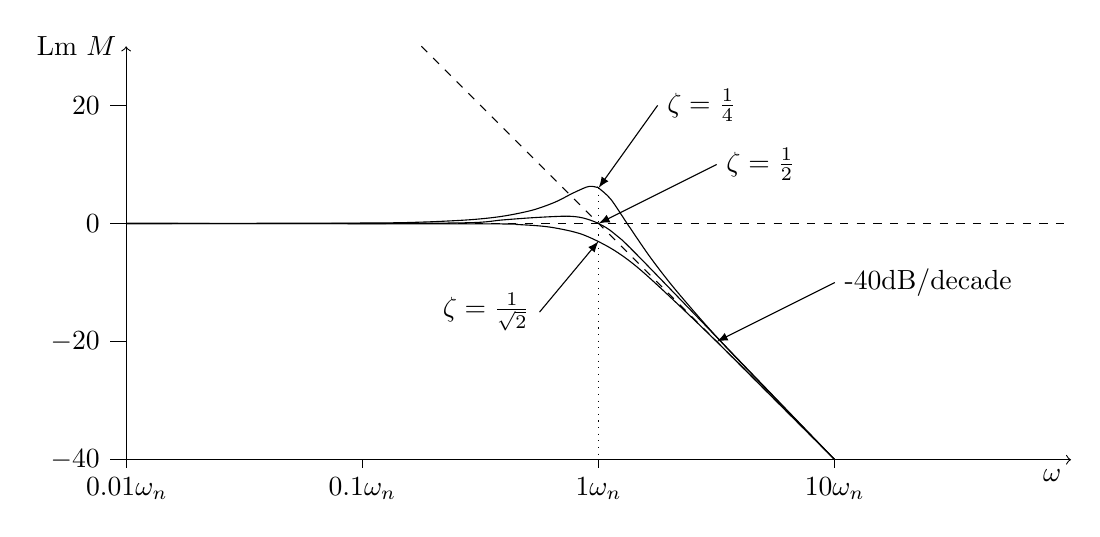
\begin{tikzpicture}[scale=1.5,xscale=2]
	\draw[<->] (0,3.5) node[left] {$\Lm M$} |- (4,0) node[below left] {$ \omega $};
	
	\foreach \x [evaluate=\x as \xeval using log10(\x)+2] in {0.01,0.1,1,10} \draw (\xeval cm,0pt) -- (\xeval cm,-2pt) node[anchor=north] {${\x\omega_n}$};
	
	\foreach \y [evaluate=\y as \yeval using (\y+40)/20] in {-40,20,0,-20} \draw (0pt,\yeval cm) -- (-2pt,\yeval cm) node[anchor=east] {$\y$};
	
	\draw[dashed] (0,2) -- (4,2);
	\draw[dashed] (1.25,3.5) -- (3,0);
	\draw[dotted] (2,2.301) -- (2,0);
	\draw plot [smooth] coordinates { (0,2) (1.5,1.997) (1.66,1.991) (1.796,1.969) (1.932,1.907) (2.068,1.771) (2.204,1.561) (2.5,1) (3,0) };
	\draw plot [smooth] coordinates { (0,2) (1,2) (1.456,2.007) (1.592,2.03) (1.728,2.05) (1.864,2.062) (1.932,2.048) (2,2) (2.068,1.912) (2.204,1.651) (3,0) };
	\draw plot [smooth] coordinates { (0,2) (1,2.004) (1.252,2.012) (1.456,2.032) (1.592,2.061) (1.718,2.112) (1.816,2.181) (1.89,2.256) (1.948,2.308) (1.971,2.315) (1.994,2.306) (2,2.301) (2.052,2.205) (2.126,1.985) (2.224,1.7) (2.34,1.405) (2.544,0.9445) (3,0) };
	\draw[-latex] (3,1.5) node[right] {-40dB/decade} -- (2.5,1);
	\draw[-latex] (2.25,3) node[right] {$ \zeta=\frac{1}{4} $} -- (2,2.301);
	\draw[-latex] (2.5,2.5) node[right] {$ \zeta=\frac{1}{2} $} -- (2,2);
	\draw[-latex] (1.75,1.25) node[left] {$ \zeta=\frac{1}{\sqrt{2}} $} -- (2,1.85);
	\end{tikzpicture}
	
%	\begin{tikzpicture}
%		\begin{scope}[trim axis left,trim axis right]
%		\begin{semilogxaxis}[title=Bode Diagram, ylabel=Magnitude (dB), xmin=1e-2, xmax=1e2, ymin=-40, ymax=30, xticklabels={$ 0.001\omega_n $,$ 0.01\omega_n $,$ 0.1\omega_n $,$ \omega_n $,$ 10\omega_n $},yticklabels={-60, -40,-20,-0,20}, width=0.8\textwidth,height=6cm,xshift=-1cm];
%		\addplot[thick,domain=1e-2:1e0] {40+20*log10(x)};
%		\addplot[thick,domain=1e0:1e2] {40};
%		\end{semilogxaxis}
%		\end{scope}
%	\end{tikzpicture}
\end{center}
Next, we find the phase as a function of $ \omega $.
\[ \phi = -\tan^{-1} \left( \frac{2\zeta\frac{\omega}{\omega_n}}{1-\frac{\omega^2}{\omega_n^2}} \right) \]
From here, we will find $ \phi $ when $ \frac{\omega}{\omega_n} = 1 $ precisely and find approximations for $ \phi $ when $ \frac{\omega}{\omega_n} \ll 1 $ and when $ \frac{\omega}{\omega_n} \gg 1 $. 
\begin{itemize}
	\item When $ \frac{\omega}{\omega_n} \ll 1 $ (meaning $ \omega\to 0 $), $ \phi\approx -\tan^{-1}(\frac{0}{1})=0^\circ$
	\item When $ \omega = \omega_n $, $ \phi\approx -\tan^{-1}(\frac{2\zeta}{0})=-90^\circ $
	\item When $ \frac{\omega}{\omega_n} \gg 1 $ (meaning $ \omega\to \infty $), $ \phi\approx -\tan^{-1}(\frac{2\zeta}{-\infty})=-180^\circ $
\end{itemize}
Decreasing $ \zeta $ decreases the range of frequencies over which the phase shift occurs --- that is, the phase shift is ``sharper'', and the slope at the center ($ \omega=\omega_n $) is closed to vertical. When drawing a 2nd-order phase plot by hand, the phase shift can be approximated by estimating that the phase shift starts at
\[ \omega_{start} = \omega_n \cdot 10^{-\zeta} \] 
and ends at
\[ \omega_{end} = \omega_n \cdot 10^{\zeta} \]
More simply, this means that the phase change takes place over $ 2\zeta $ decades. For example,
\begin{itemize}
	\item If $ \zeta = 1/2 $, the phase shift happens over 1 decade --- half a decade for $ 0^\circ $ to $ -90^\circ $, and half a decade for $ -90^\circ $ to $ -180^\circ $.
	\item If $ \zeta = 1/4 $, the phase shift happens over half a decade --- one quarter of a decade for $ 0^\circ $ to $ -90^\circ $, and one quarter of a decade for $ -90^\circ $ to $ -180^\circ $.
\end{itemize}
\begin{center}
	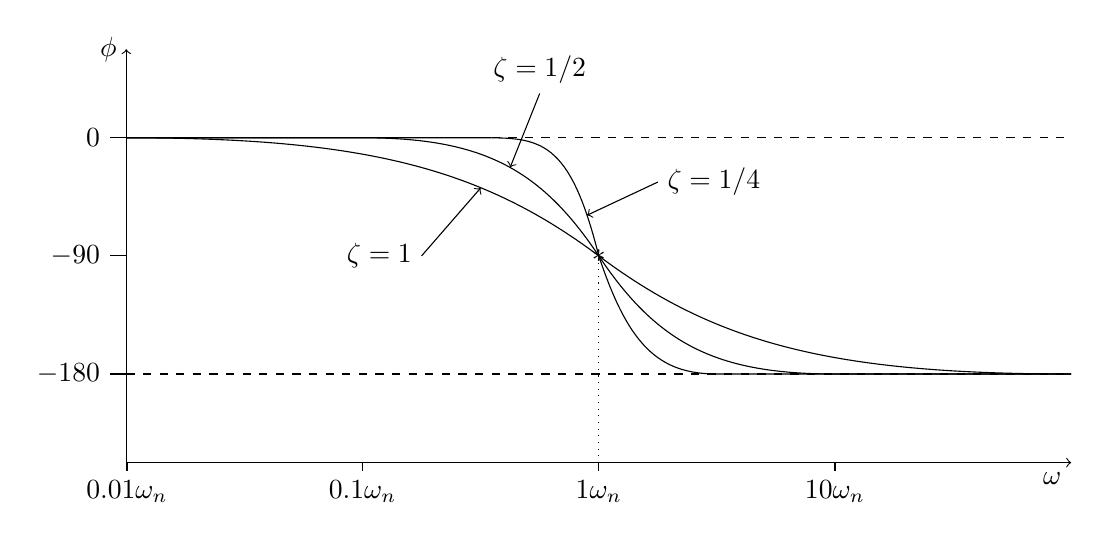
\begin{tikzpicture}[scale=1.5,xscale=2]
	\draw[<->] (0,3.5) node[left] {$\phi$} |- (4,0) node[below left] {$ \omega $};
	
	\foreach \x [evaluate=\x as \xeval using log10(\x)+2] in {0.01,0.1,1,10} \draw (\xeval cm,0pt) -- (\xeval cm,-2pt) node[anchor=north] {${\x}{\omega_n}$};
	
	\foreach \y [evaluate=\y as \yeval using (\y+180)/90+.75] in {-180,-90,0} \draw (0pt,\yeval cm) -- (-2pt,\yeval cm) node[anchor=east] {$\y$};
	
	\draw (0,2.75) ..controls (1,2.75) and (1.5,2.5) .. (2,1.75) ..controls (2.5,1) and (3,.75) .. (4,.75);
	\draw (0,2.75) -- (1,2.75) ..controls (1.5,2.75) and (1.75,2.5) .. (2,1.75) ..controls (2.25,1) and (2.5,.75) .. (3,.75) -- (4,.75);
	\draw (0,2.75) -- (1.5,2.75) ..controls (1.75,2.75) and (1.875,2.75) .. (2,1.75) ..controls (2.125,1) and (2.25,.75) .. (2.5,.75) -- (4,.75);
	\draw[dashed] (0,0.75) -- (4,0.75);
	\draw[dashed] (0,2.75) -- (4,2.75);
%	\draw[dashed] (1,2.75) -- (3,0.75);
%	\draw[dashed] (1.5,2.75) -- (2.5,0.75);
%	\draw[dashed] (1.75,2.75) -- (2.25,0.75);
	%	\draw[dashed] (1,0) -- (1,2);
	%	\draw[dashed] (3,0) -- (3,1);
	\draw[dotted] (2,1.75) node {$ * $} -- (2,0); % node[above right] {$ -90^\circ $}
%	\draw[-latex] (1.6875,1.875) -- (2.0625,2.375) node[right] {Increasing $ \zeta $};

	\draw[->] (1.25,1.75) node[left] {$ \zeta=1 $} -- (1.5,2.325);
	\draw[->] (1.75,3.125) node[above] {$ \zeta=1/2 $} -- (1.625,2.5);
	\draw[->] (2.25,2.375) node[right] {$ \zeta=1/4 $} -- (1.95,2.09375);
	\end{tikzpicture}
\end{center}

\end{document}

